\documentclass{article}

\title{Fractional Curvature Calculations}
\usepackage{dztex}
\usepackage{mathtools}
\usepackage{IEEEtrantools}

\renewcommand{\familydefault}{\sfdefault}
\DeclareMathOperator{\diam}{diam}
\DeclareMathOperator{\hm}{\mathcal{H}}
\DeclareMathOperator{\betop}{\mathcal{B}}
\DeclareMathOperator{\gamop}{\Gamma}
\newcommand{\bet}[1]{\betop\parens{#1}}
\newcommand{\gam}[1]{\gamop\parens{#1}}
\newcommand{\aeven}{\mathcal{A}_{\mathrm{even}}^+}
\newcommand{\aodd}{\mathcal{A}_{\mathrm{odd}}^+}
\newcommand{\bec}[1]{\mathbf{#1}}
\newcommand{\ud}{\mathrm{d}}
\newcommand{\eqlbl}[1]{\opstack{=}{#1}}
\newcommand{\opstack}[2]{\stackrel{\mathclap{\normalfont\tiny \mbox{#2}}}{#1}}

\usepackage{pgfplots}
\pgfplotsset{compat=1.5.1}
\pgfplotsset{every tick label/.append style={font=\footnotesize}}


\begin{document}

\subsection{Introduction} Here I will collect calculations done while exploring fractional curvature.

\subsection{$\kappa_\sigma$ of the unit circle}
We wish to compute
$$
\kappa_\sigma(z) := \parens{\int_{\aeven} - \int_{\aodd}} \frac{\parens{\bec{a} \cdot \bec{t}(z)} \bec{b} - \parens{\bec{b} \cdot \bec{t}(z)}\bec{a}}{r^{1+\sigma}} \, d\mathcal{H}^{2}\parens{\bec{a}, \bec{b}, r}
$$
for $C$ given by
$$
z(\phi) = \parens{\cos \phi, \sin \phi}, \phi \in [0, 2\pi].
$$
Due to symmetry $\kappa_\sigma(z(0)) = \kappa_\sigma(z(\phi)) \, \forall \phi \in (0, 2\pi]$, so we can focus on the case when $z = (1, 0)$. We have $\bec{t}(z) = (0, 1)$. 
in order to help us characterize $\aeven, \aodd$:
\begin{IEEEeqnarray*}{rCl}
  \prescript{1}{}{\aeven} &=& \braces{
    \parens{\begin{pmatrix} \cos\phi \\ \sin\phi\end{pmatrix}, \begin{pmatrix} -\sin\phi \\ \cos\phi \end{pmatrix}, r} \mid \phi \in \bracp{\frac{3\pi}{2}, 2\pi} \cup \bracp{0, \frac{\pi}{2}}, r \in [0, \infty)
  } \\
  \prescript{2}{}{\aeven} &=& \braces{
    \parens{\begin{pmatrix} \cos\phi \\ \sin\phi\end{pmatrix}, \begin{pmatrix} \sin\phi \\ -\cos\phi \end{pmatrix}, r} \mid \phi \in \bracp{\frac{\pi}{2}, \frac{3\pi}{2}}, r \in [0, \cos \parens{\pi - \phi})
  } \\
  \aeven &=& \prescript{1}{}{\aeven} \cup \prescript{2}{}{\aeven} \\
  \aodd &=& \braces{
    \parens{\begin{pmatrix} \cos\phi \\ \sin\phi\end{pmatrix}, \begin{pmatrix} \sin\phi \\ -\cos\phi \end{pmatrix}, r} \mid \phi \in \bracp{\frac{\pi}{2}, \frac{3\pi}{2}}, r \in [\cos \parens{\pi - \phi}, \infty)
  } \\
\end{IEEEeqnarray*}
These subsets are motivated by the following picture:
\begin{center}
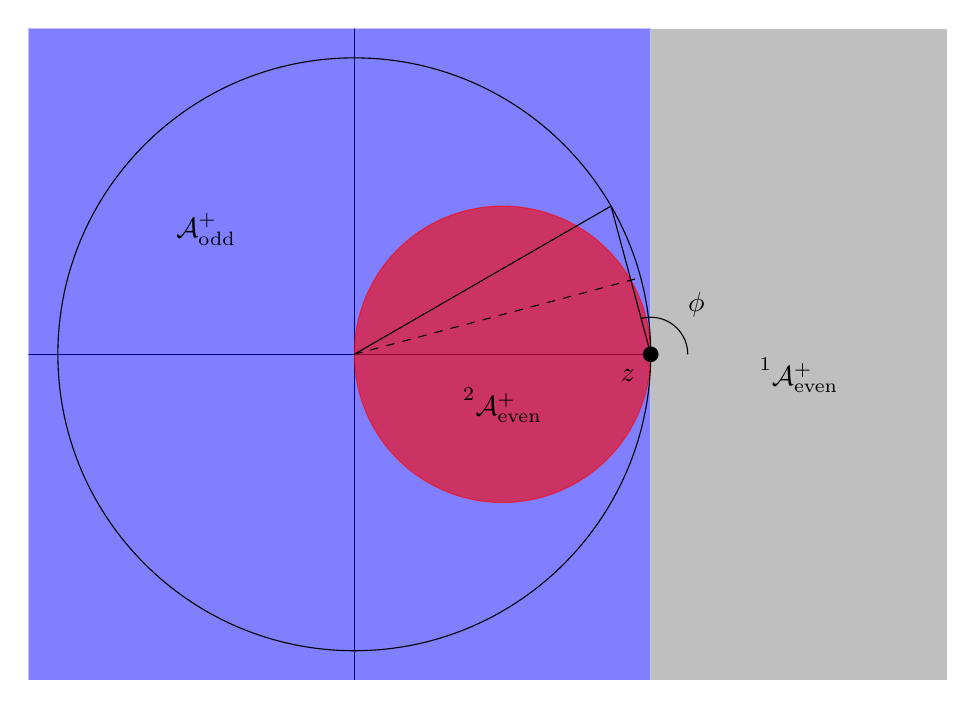
\begin{tikzpicture}
\begin{axis}[ 
    axis lines = middle,
    ticks = none,
    axis line style={-},
    ymin=-1.1, ymax=1.1,
    xmin=-1.1, xmax=2,
    axis equal image,
    height=4.5in
]
\draw[color=white, fill = lightgray] (axis cs:1, -1.1) rectangle (axis cs:2, 1.1);

\draw[color=white, fill = blue, opacity=0.5] (axis cs:-1.1, -1.1) rectangle (axis cs:1, 1.1);
\addplot[data cs=polar, red, opacity=0.6, domain=90:270,samples=180,smooth, fill=red, fill opacity=0.6] (x, {cos(x)});

\node[label={{$\prescript{1}{}{\aeven}$}}] at (axis cs:1.5,-0.2) {};
\node[label={{$\prescript{2}{}{\aeven}$}}] at (axis cs:0.5,-0.3) {};
\node[label={{$\aodd$}}] at (axis cs:-0.5,0.3) {};

\draw (axis cs:0,0) circle [radius=1];
\node[label={225:{$z$}},circle,fill,inner sep=2pt] at (axis cs:1,0) {};

\draw (axis cs:0,0) -- (axis cs:{cos(30)},{sin(30)});
\draw (axis cs:1,0) -- (axis cs:{cos(30)},{sin(30)});
\draw[dashed] (axis cs:0,0) -- (axis cs:{cos(15)},{sin(15)});

\draw (axis cs:1.125,0.0) arc(0:{90+15}:{transformdirectionx(0.125)}) (axis cs:{1-0.125},0);
\node[label={45:{$\phi$}}] at (axis cs:1.06,0.06) {};
\end{axis}
\end{tikzpicture}
\end{center}
Before jumping into calculations observe that we can parameterize our subset of $\mathbb{R}^5$ via $(\theta, r)$, as shown in the definition of the subsets above and put 
$$
s(\theta) = \begin{cases}
  -1 & \theta \in [\pi/2, 3\pi/2] \\
  1 & \textup{otherwise}
\end{cases}.
$$
We can simplify our integrand as follows:
\begin{IEEEeqnarray*}{rCl}
  J(r, \theta) &=& \frac{\parens{\bec{a} \cdot \bec{t}(z)} \bec{b} - \parens{\bec{b} \cdot \bec{t}(z)}\bec{a}}{r^{1+\sigma}} \\
  &=& \frac{
    \parens{\begin{pmatrix} \cos\theta \\ \sin\theta \end{pmatrix} \cdot \begin{pmatrix} 0 \\ 1 \end{pmatrix}}s(\theta) \begin{pmatrix} -\sin \theta \\ \cos \theta \end{pmatrix}
    - \parens{s(\theta)\begin{pmatrix} -\sin\theta \\ \cos\theta \end{pmatrix} \cdot \begin{pmatrix} 0 \\ 1 \end{pmatrix}}s(\theta) \begin{pmatrix} \cos \theta \\ \sin \theta \end{pmatrix}
    }{r^{1+\sigma}} \\
    &=& \frac{s(\theta) \parens{\sin\theta \begin{pmatrix} -\sin \theta \\ \cos \theta \end{pmatrix} - \cos\theta \begin{pmatrix} \cos \theta \\ \sin \theta \end{pmatrix}}}{r^{1+\sigma}} = \frac{-s(\theta) \begin{pmatrix} \sin^2\theta + \cos^2\theta \\ -\sin\theta\cos\theta + \cos\theta\sin\theta \end{pmatrix}}{r^{1+\sigma}} \\
      &=& \begin{pmatrix} -1 \\ 0 \end{pmatrix} \frac{s(\theta)}{r^{1+\sigma}}
\end{IEEEeqnarray*}
Next we can start computing integrals, we begin by integrating over $\aeven$:
\begin{IEEEeqnarray*}{rCl}
  \int_{\aeven} \frac{s(\theta)}{r^{1+\sigma}} \, d\mathcal{H}^2(r, \theta) &=& \parens{\int_{3\pi/2}^{2\pi} + \int_{0}^{\pi/2}} \int_\epsilon^\infty \frac{s(\theta)}{r^{1+\sigma}} \, dr \, d\theta + \int_{\pi/2}^{3\pi/2} \int_{\epsilon}^{\cos(\pi-\theta)} \frac{s(\theta)}{r^{1+\sigma}} \, dr \, d\theta \\
  &=& \parens{\int_{3\pi/2}^{2\pi} + \int_{0}^{\pi/2}} \int_\epsilon^\infty \frac{1}{r^{1+\sigma}} \, d r \, d\theta - \int_{\pi/2}^{3\pi/2} \int_{\epsilon}^{\cos(\pi-\theta)} \frac{1}{r^{1+\sigma}} \, dr \, d\theta \\
  &=& -\frac{1}{\sigma}\parens{\int_{3\pi/2}^{2\pi} + \int_{0}^{\pi/2}} \parens{ 0 - \frac{1}{\epsilon^\sigma} } \, d\theta + \frac{1}{\sigma} \int_{\pi/2}^{3\pi/2} \parens{\frac{1}{\parens{\cos(\pi-\theta)}^\sigma} - \frac{1}{\epsilon^\sigma}} \, d \theta \\
  &=& \frac{\pi}{\sigma\epsilon^\sigma} - \frac{\pi}{\sigma\epsilon^\sigma} - \frac{1}{\sigma} \int_{\pi/2}^{-\pi/2} \parens{\sec \theta}^\sigma \, d\theta \\
  &=& \frac{1}{\sigma} \int_{-\pi/2}^{\pi/2} \parens{\sec \theta}^\sigma \, d \theta.
\end{IEEEeqnarray*}
Now for $\aodd$:
\begin{IEEEeqnarray*}{rCl}
  \int_{\aodd} \frac{s(\theta)}{r^{1+\sigma}} \, d\mathcal{H}^2(r, \theta) &=& \int_{\pi/2}^{3\pi/2} \int_{\cos(\pi - \theta)}^\infty \frac{s(\theta)}{r^{1+\sigma}} \, dr \, d\theta \\
  &=& - \int_{\pi/2}^{3\pi/2} \int_{\cos(\pi - \theta)}^\infty \frac{1}{r^{1+\sigma}} \, dr \, d\theta \\
  &=& \frac{1}{\sigma} \int_{\pi/2}^{3\pi/2} \parens{0 - \frac{1}{\parens{\cos(\pi - \theta)}^\sigma}} \, d\theta \\
  &=& \frac{1}{\sigma}\int_{\pi/2}^{-\pi/2} \parens{\sec \theta}^\sigma \, d \theta \\
  &=& -\frac{1}{\sigma}\int_{-\pi/2}^{\pi/2} \parens{\sec \theta}^\sigma \, d\theta.
\end{IEEEeqnarray*}
Putting these computations together we have:
\begin{IEEEeqnarray*}{rl}
  \parens{\int_{\aeven} - \int_{\aodd}}& \frac{\parens{\bec{a} \cdot \bec{t}(z)} \bec{b} - \parens{\bec{b} \cdot \bec{t}(z)}\bec{a}}{r^{1+\sigma}} \, d\mathcal{H}^{2}\parens{\bec{a}, \bec{b}, r} \\
   &= \parens{\int_{\aeven} - \int_{\aodd}} \begin{pmatrix} -1 \\ 0 \end{pmatrix} \frac{s(\theta)}{r^{1+\sigma}} \, d\mathcal{H}^2 \\
   &= \begin{pmatrix} -1 \\ 0 \end{pmatrix} \parens{\frac{1}{\sigma} \int_{-\pi/2}^{\pi/2} \parens{\sec \theta}^\sigma \, d\theta + \frac{1}{\sigma} \int_{-\pi/2}^{\pi/2} \parens{\sec \theta}^\sigma \, d\theta} \\
   &= \begin{pmatrix} -1 \\ 0 \end{pmatrix} \frac{2}{\sigma} \int_{-\pi/2}^{\pi/2} \parens{\sec \theta}^\sigma \, d\theta \\
     &= \begin{pmatrix} -1 \\ 0 \end{pmatrix} \frac{2\sqrt{\pi}\gam{\frac{1-\sigma}{2}}}{\sigma\gam{1-\frac{\sigma}{2}}} \textup{ by \eqref{l2}}.
\end{IEEEeqnarray*}
Finally we can recover the classical curvature $\kappa = z''(0) = (-1, 0)$ as follows:
\begin{IEEEeqnarray*}{rCl}
  \lim_{\sigma \uparrow 1} \frac{\parens{1 - \sigma}}{4} \kappa_\sigma &=& \lim_{\sigma\uparrow 1} \begin{pmatrix} -1 \\ 0 \end{pmatrix} \frac{2\parens{1-\sigma}\sqrt{\pi} \gam{\frac{1-\sigma}{2}}}{4\sigma \gam{1-\frac{\sigma}{2}}} \\
    &=& \begin{pmatrix} -1 \\ 0 \end{pmatrix} \frac{\sqrt{\pi}}{2} \lim_{\sigma \uparrow 1} \frac{\parens{1-\sigma}\gam{\frac{1-\sigma}{2}}}{\sigma \gam{1 - \frac{\sigma}{2}}} \\
      &=& \begin{pmatrix} -1 \\ 0 \end{pmatrix} \frac{1}{2} \underbrace{\lim_{\sigma\uparrow 1} \parens{1-\sigma} \gam{\frac{1-\sigma}{2}}}_{\eqref{l3}} = \begin{pmatrix} -1 \\ 0 \end{pmatrix} = \kappa.
\end{IEEEeqnarray*}

\subsection{Definitions \& Properties}
For the sake of completeness we use the following definitions are used:
\begin{IEEEeqnarray}{rCl}
  \gam{z} &=& \int_0^\infty t^{z-1} e^{-t} \, dt \textup{ where } \Re(z) > 0, \label{d1} \\
  \bet{z_1, z_2} &=& \int_0^1 t^{z_1 - 1} \parens{1-t}^{z_2-1} \, dt \textup{ where } \Re(z_1), \Re(z_2) > 0. \label{d2}
\end{IEEEeqnarray}
And we will assume the following properties:
\begin{IEEEeqnarray}{rCl}
  \bet{z_1, z_2} &=& \frac{\gam{z_1}\gam{z_2}}{\gam{z_1+z_2}}, \label{p1} \\
  \gam{z}\gam{1-z} &=& \frac{\pi}{\sin \parens{\pi z}}. \label{p2}
\end{IEEEeqnarray}
The former can be shown via a direct computation of the product $\gam{z_1}\gam{z_2}$ and change of variables \& the latter via Weierstrass products.
\newpage
\subsection{Calculations}
\begin{lemma}\label{l1}
  $$
  \gam{\frac{1}{2}} = \sqrt{\pi}
  $$
\end{lemma}
\begin{proof}
  From \eqref{p2} we have:
  $$
  \parens{\gam{\frac{1}{2}}}^2 = \gam{\frac{1}{2}} \gam{\frac{1}{2}} = \frac{\pi}{\sin\parens{\frac{\pi}{2}}} = \pi.
  $$
\end{proof}
\begin{lemma}\label{l2}
  $$
  \int_{-\pi/2}^{\pi/2} \parens{\cos\theta}^{-\sigma} \, d \theta = \frac{\sqrt{\pi}\gam{\frac{1-\sigma}{2}}}{\gam{1-\frac{\sigma}{2}}} \textup{ for } \sigma \in (0, 1)
  $$
\end{lemma}
\begin{proof}
  Beginning with \eqref{d2} and using a change of variables $t \to \sin^2 \theta$ so that $1 - t = \cos^2 \theta$ and $dt = 2\sin\theta \cos\theta \, d\theta$, thus
  $$
  \bet{z_1, z_2} = \int_0^{\pi/2} \parens{\sin \theta}^{2z_1 - 2} \parens{\cos \theta}^{2z_2 - 2} \cdot 2 \sin\theta\cos\theta \, d\theta = 2\int_0^{\pi/2} \parens{\sin \theta}^{2z_1-1} \parens{\cos\theta}^{2z_2 - 1} \, d\theta.
  $$
  Now, since $\frac{1-\sigma}{2} > 0$ when $\sigma < 1$ we have:
  $$
  \bet{\frac{1}{2}, \frac{1-\sigma}{2}} = 2\int_0^{\pi/2} \parens{\sin \theta}^{0} \parens{\cos\theta}^{1 - \sigma - 1} \, d\theta = 2\int_0^{\pi/2} \parens{\cos\theta}^{-\sigma} \, d\theta = \int_{-\pi/2}^{\pi/2} \parens{\cos\theta}^{-\sigma} \, d\theta.
  $$
  Notice the final equality comes from the fact that $\cos\theta$ is even. On the other hand, by \eqref{p1} we know
  $$
  \bet{\frac{1}{2}, \frac{1-\sigma}{2}} = \frac{\gam{1/2}\gam{\frac{1-\sigma}{2}}}{\gam{\frac{1}{2} + \frac{1-\sigma}{2}}}.
  $$
  Leveraging \eqref{l1} we find our desired equality.
\end{proof}
\begin{lemma}\label{l3}
  $$
  \lim_{\sigma\uparrow 1} \parens{1-\sigma} \gam{\frac{1-\sigma}{2}} = 2.
  $$
\end{lemma}
\begin{proof}
  By \eqref{p2} we know
  $$
  \gam{\frac{1-\sigma}{2}} = \frac{\pi}{\sin\parens{\pi \frac{1-\sigma}{2}}} \cdot \frac{1}{\gam{\frac{1+\sigma}{2}}}.
  $$
  Thus we have
  \begin{IEEEeqnarray*}{rCl}
    \lim_{\sigma\uparrow 1} \parens{1-\sigma} \gam{\frac{1-\sigma}{2}} &=& \lim_{\sigma \uparrow 1} \frac{\parens{1-\sigma}\pi}{\sin\parens{\pi \frac{1-\sigma}{2}}} \cdot \frac{1}{\gam{\frac{1+\sigma}{2}}} = \parens{\lim_{\sigma \uparrow 1} \frac{\parens{1-\sigma}\pi}{\sin\parens{\pi \frac{1-\sigma}{2}}}} \cdot \parens{\lim_{\sigma\uparrow 1} \frac{1}{\gam{\frac{1+\sigma}{2}}}} \\
    &=& \pi \lim_{\sigma \uparrow 1} \frac{\parens{1-\sigma}}{\sin\parens{\pi \frac{1-\sigma}{2}}} \underbrace{= \pi \lim_{\sigma\uparrow 1} \frac{-1}{\cos\parens{\pi\frac{1-\sigma}{2}}\cdot \frac{-\pi}{2}}}_{\text{L'Hôpital's rule}} = 2
  \end{IEEEeqnarray*}
\end{proof}
\end{document}
